%Modelo de apresentação de pré-projeto e TCC para o curso de Tecnologia em Sistemas para Internet
%do Instituto Federal de Educação, Ciência e Tecnologia do Tocantins.
%Necessário o pacote latex-beamer instalado.
%Em distribuições Linux Debian use: sudo apt-get install latex-beamer
%@author Prof. Manoel Campos da Silva Filho - http://manoelcampos.com
%@version 1.0

\documentclass[slidestop,compress,mathserif]{beamer}
\usepackage[brazil]{babel}

\usepackage{verbatim} % http://devdaily.com/blog/post/latex/multi-line-comments-in-latex-begin-123-comment-125-verbatim
\usepackage[utf8]{inputenc}
\DeclareGraphicsExtensions{.jpg,.pdf,.mps,.png,.gif, .eps}
\usepackage{hyperref}
\usepackage{url}

\usetheme{IFTO}

\title{Título do Projeto}
\author{Nome do Aluno\inst{1} \and \\Orientador: Nome do Orientador\inst{1}}

\institute{\inst{1}Instituto Federal de Educação, Ciência e Tecnologia do Tocantins (IFTO/Palmas)}
\logo{
\includegraphics[scale=.2]{logo-ifto-completo.png}}

\setbeamertemplate{footline}[frame number]

%apenas se for usar o compilador xetex
%\usepackage{fontspec}
%\usepackage{xltxtra,xunicode}
%\defaultfontfeatures{Mapping=tex-text}
%\setromanfont[Mapping=tex-text]{Times New Roman}
%\setsansfont[Scale=MatchLowercase,Mapping=tex-text]{Gill Sans}
%\setmonofont[Scale=MatchLowercase]{Andale Mono}


\usepackage{graphicx}
\usepackage{caption}

\usepackage{listingsutf8} %listings

\lstset{
  extendedchars=true,
  numbers=left,
  stepnumber=1,
  firstnumber=1,
  numberstyle=\tiny,
  breaklines=true,
  frame=TB,
  basicstyle=\footnotesize,
  stringstyle=\ttfamily,
  showstringspaces=false,
  %backgroundcolor=\color{gray}
}

\renewcommand{\lstlistingname}{Código Fonte}
\renewcommand{\lstlistlistingname}{Lista de Códigos Fonte}

\begin{document}

\frame{
  \titlepage
} 

\begin{frame}[allowframebreaks] %Permite que o roteiro seja quebrado em vários slides
  \frametitle{Roteiro}
  \begin{center}
\includegraphics[scale=0.2]{imgs/java.png}\end{center}
  %\setcounter{tocdepth}{1} %Exibe apenas os elementos de primeiro nível no sumário
  \tableofcontents
\end{frame}

%\frame{\frametitle{Roteiro} %Roteiro sem quebra de página
%  \begin{center}
\includegraphics[scale=0.2]{imgs/java.png}\end{center}
%  %\setcounter{tocdepth}{1} %Exibe apenas os elementos de primeiro nível no sumário
%  \tableofcontents
%}


%Cria um tópico (que pode conter vários slides)
\section[Plataforma]{Plataforma Java}

%Cria um sub-tópico
\subsection{Apresentação}

%Cria um slide para o tópico/sub-tópico atuals
\frame{\frametitle{Plataforma Java - Apresentação}
\begin{itemize}
  \item Multi-linguagem. Tem como principal a linguagem Java
  \item Permite que aplicações desenvolvidas sejam executadas em diferentes hardwares e sistema operacionais 
  \item Necessidade de uma Máquina Virtual Java (Java Virtual Machine - JVM/Java Runtime Environment - JRE) para execução de aplicações
  \item JVM específica para cada hardware e SO
\end{itemize}  
}

%Outro slide
\frame{\frametitle{Plataforma Java - Apresentação}
\begin{itemize}
  \item Bytecodes (.class): interpretados pela JVM. Compilados a partir dos arquivos fonte
  (normalmente arquivos .java)
  \item Just In Time Compiler (JIT): compilação de bytecodes para código de máquina na primeira execução
\end{itemize}
\begin{center}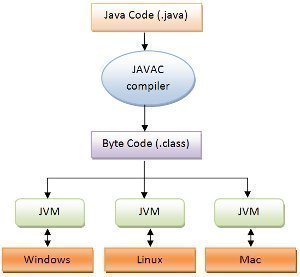
\includegraphics[scale=0.3]{imgs/Java-Bytecode.png}\end{center} 
Imagem: \url{http://www.tech-faq.com/java-bytecode.html}
}

%Cria um sub-sub tópico
\subsubsection{Edições}

%Cria um slide para o tópico anterior
\frame{\frametitle{Plataforma Java - Edições}
\begin{itemize}
  \item Java Standard Edition - JSE (antiga J2SE): plataforma base para o desenvolvimento de aplicações de uso geral em Java, como aplicações console ou desktop.
  \item Java Enterprise Edition - JEE (antiga J2EE): plataforma para o desenvolvimento de aplicações de Web
  \item Java Micro Edition - JME (antiga J2ME): plataforma para o desenvolvimento de aplicações para sistemas embarcadas (como celulares, smartphones e TV's).
  \begin{itemize}
  \item Perdeu mercado p/ novas plataformas (iPhone, Android, Windows Phone ...)
  \end{itemize}
  \item Java Card: plataforma para desenvolvimento de aplicações embarcadas em cartões 
  (como cartões de crédito com chip, SIM Cards, etc) e dispositivos
  extremamente restritos de recursos de hardware.
\end{itemize}
}

%Cria outro sub-sub tópico
\subsubsection{Linguagens}

%Cria um slide para o tópico anterior
\frame{\frametitle{Plataforma Java - Linguagens}
\begin{itemize}
  \item Não restrita ao uso da linguagem Java. Algumas linguagens que podem ser utilizadas:
  \begin{itemize}
  \item Groovy
  \item Ruby (usando JRuby)
  \item Python (usando Jython)
  \item JavaScript (usando Rhino)
  \end{itemize}
\end{itemize}
}
      

%Cria outro sub-sub tópico
\subsubsection[Dev/Exec]{Desenvolvimento e Execução}

%Cria um slide para o tópico anterior
\frame{\frametitle{Plataforma Java - Desenvolvimento e Execução}
\begin{itemize}
  \item Java Development Kit (JDK): contém ferramentas básicas para desenvolvimento de aplicações Java. Alguns itens do JDK:
  \begin{itemize}
  \item javac – Compilador bytecode
  \item java – Interpretador de bytecodes (.class)
  \item javadoc – Geração de documentação (em HTML) de aplicações Java
  \item jar – Empacotador de aplicações Java
  \item javap – Descompilador de arquivos .class
  \item javaws – Java Web Start para execução de aplicações JNLP
  \end{itemize}
  \item Java Runtime Environment (JRE): contém a JVM para execução de aplicações desenvolvidas para a plataforma Java  
\end{itemize}
}

%Cria outro slide para o tópico anterior
\frame{\frametitle{Plataforma Java - Desenvolvimento e Execução}
\begin{itemize}
  \item Devido às suas especificações livres, surgiram implementações
da comunidade:
  \begin{itemize}
  \item Open JDK / Open JRE
  \item GNU Compiler for Java: GCJ
  \end{itemize}
\end{itemize}
}

\subsection[Linguagem]{Linguagem Java}

\subsubsection{Características}
\frame{\frametitle{Linguagem Java - Características}

\begin{itemize}
  \item Desenvolvida inicialmente pela Sun Microsystems (atual Oracle)
  \item Alto Nível
  \item Fortemente Tipada
  \item Case Sensitive
  \item Multiplataforma. Slogan inicial: Write once run anywhere
  \item Desenvolvimento Desktop, Web e Mobile  
  \item Orientada a Objetos: dados e funções em um mesmo lugar  
  \item Linguagem de uso livre, totalmente Open Source a partir de 2007
  \item Amplamente utilizada: \url{www.tiobe.com/content/paperinfo/tpci/}
  \item Garbage Collection (Coleta de Lixo)
\end{itemize}
}

\subsubsection[IDE's]{Ambientes de Desenvolvimento (IDE's)}
\frame{\frametitle{Linguagem Java - Ambientes de Desenvolvimento}
\begin{itemize}
  \item Integrated Development Environment - IDE (Ambiente Integrado de Desenvolvimento): 
  ambientes profissionais e livres 
  \begin{itemize}
  \item Eclipse: \url{www.eclipse.org}
  \item Netbeans: \url{www.netbeans.org}
  \end{itemize}
\end{itemize}
}

\section[Introdução Java]{Introdução à Linguagem Java}

\subsection[Hello]{Hello World}

\begin{frame}[allowframebreaks]
  \frametitle{Hello World em Java}
      
  \lstinputlisting[caption=Hello World em Java, label=list:hello, language=java, 
  style=colorful, style=numbered]{src/Hello.java}
\end{frame}



%\lstinputlisting[language=TeX, label=exemplo1, caption={``Olá mundo em LaTeX''}]{ola_mundo.tex}

\end{document}
